\label{timeline}
Given the size of the problem space and that the proposed work will be performed in no more than a year, we propose to focus on three main contributions:
\begin{inparaenum}[(1)]
\item evaluating and deriving the makespan for a campaign as a set of independent static O(10) workflows with heterogeneous resource requirements provided by ecological and biomolecular sciences use cases on dynamic resources; 
\item offering execution planning capabilities to minimize the makespan of a campaign; and 
\item validating our planning capability by executing the workflows of our use cases and measuring the accuracy of the estimated campaign runtime and planned execution compared to a random plan.
\end{inparaenum}
In addition, we will explore the requirements to support campaigns with dynamic workflows.

To this end, we propose to achieve the following objectives with an estimation of the time needed:
\begin{enumerate}
    \item Develop a campaign manager prototype, which will derive and execute a plan. Duration 3 months
    \item Implement proposed makespan algorithm for executing a campaign from the ecological sciences. Duration 4 months. It overlaps with the last month of phase 1.
    \item Experimentally measure the performance of the selected makespan algorithm for a scientific campaign. Duration 5 months. It overlaps with objective 2 
\end{enumerate}
Figure~\ref{fig:work_plan} shows the Gantt chart of the proposed work.
Subsections~\ref{obj1},~\ref{obj2}, and~\ref{obj3} provide more details as to what will be achieved during each phase of the proposal.
In addition, we allocate three months to accommodate foreseen challenges and risks.
\begin{figure*}[t]
	\centering
	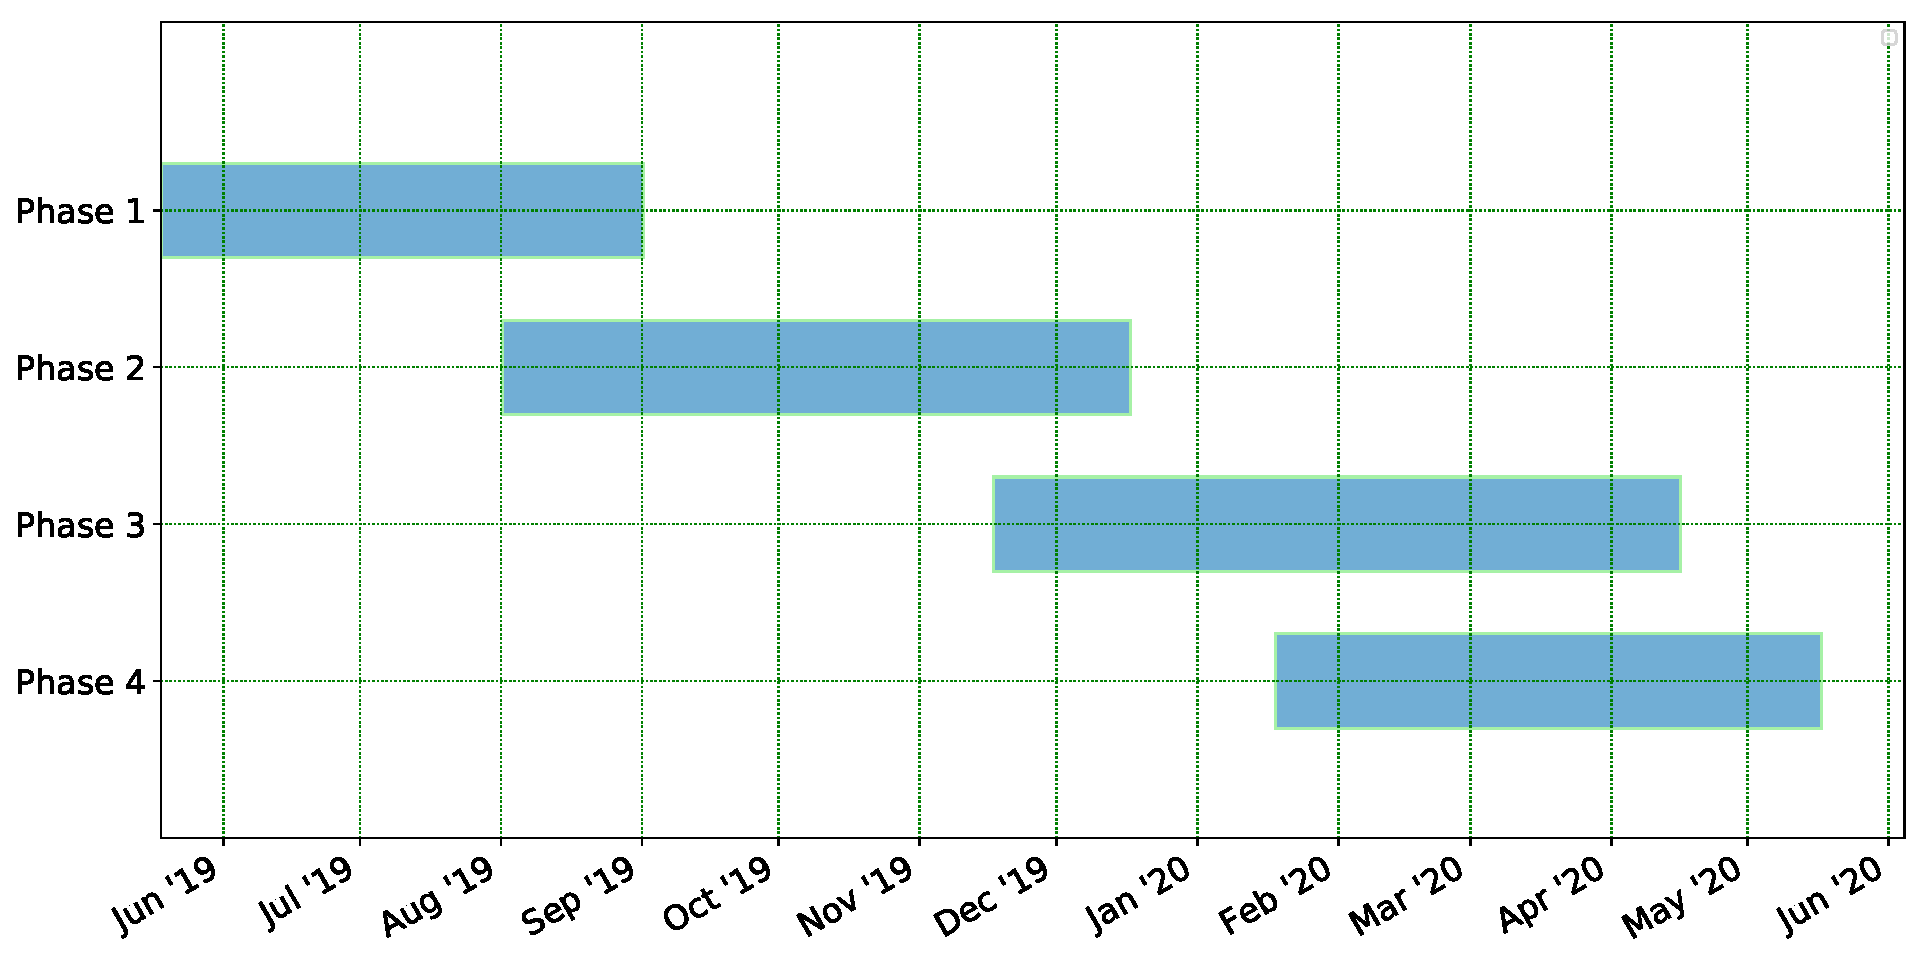
\includegraphics[width=.95\textwidth]{figures/phd_plan.pdf}
	\caption{Planned timeline of proposed research}\label{fig:work_plan}
\end{figure*}

\subsubsection{Phase 1: Design and implementation of a campaign manager}
\label{obj1}

Phase 1 would include design discussions for a prototype of the campaign manager.
Designing a prototype is an iterative process, and it will provided the basic functionality of the campaign manager.
These discussions will result to the requirements of the campaign manager and its API.

There are several methods to design a CM.
PanDA~\cite{maeno2008panda} and glideinWMS~\cite{sfiligoi2008glidein} are utilizing a dedicated server to hold workflows and schedule them to resources.
Balsam~\cite{salim2019balsam} utilizes a database to hold the campaign and workers are pulling workflow tasks for execution.
DIRAC~\cite{casajus2010dirac} creates a set of queues that hold different sized workflow tasks, and use dedicated workers for each queue.
Understanding whether existing design approaches fit the requirements of our use cases is necessary to finalize the CM design.

A prototype will be implemented and will provide campaign execution capabilities.
The prototype will be implemented in python and interface with RADICAL-EnTK as its WMF.
Initially, we will assume that the workflows of the campaign are described based on the EnTK's API.
This will allows us to quickly develop the prototype for the campaign manager.
If there is time in phase 1 we will relax this assumption and try to support different methods of describing workflows based on our use cases.
This will require to translate a workflow from any representation to EnTK's.
Furthermore, the planner component should allow the support multiple makespan algorithms.
Success of this phase will provide an installable python package. 


\subsubsection{Phase 2: Implementation and performance analysis of makespan algorithm}
\label{obj2}
Phase 2 includes implementing the proposed HEFT algorithm in the CM prototype, and characterizing its performance.
Initially, we will implement a random planner, while we extend and implement HEFT to support a campaign.
We will first use a campaign with homogeneous workflows and homogeneous resources to validate our implementation (different mappings of workflows on resources should all have the same makespan as explained in~\S\ref{sec:proposed}). We will then use heterogeneous workflows and static homogeneous resources, eventually moving to static heterogeneous resources and finally to dynamic heterogeneous resources.
This will allow us to characterize the performance of our proposed algorithm, compared to a random plan.

Preliminary experimentation during this phase will provide us with information on whether HEFT can support a campaign execution.
In case it does, we will proceed with phase 3 as soon as possible.
Otherwise, we will research algorithms that can support campaign execution and implement them, following the same approach described above. Even a negative result will be interesting, seeing the lack of current analysis about planning for campaign managers.

\subsubsection{Phase 3: Experimental performance analysis}
\label{obj3}
Phase 3 of the proposed research plan includes an experimental performance analysis of the campaign manager for a set of selected use cases.
We will execute campaigns based on our use cases, with and without our campaign manager, for different campaign sizes.
Based on the gathered data, we will measure metrics such as makespan, resource utilization.
This performance analysis will compare the execution of a computational campaign with and without our CM prototype.
This comparison will provide us with information about whether and when a CM should be used, and about whether the CM performance correlates to the size and characteristics or the campaign's workflow and available resources.

% ---------------------------------------------------------------------------
% Why
\subsection{Significance and impact of work}
Several scientific campaigns require to execute a large number of workflows several times with different input data or initial conditions. 
The required concurrency to minimize the execution time of the campaign is not necessarily constant and may change based on resource availability. 
The campaign manager suggested in this proposal will be the first that offers domain and resource agnostic campaign execution, as well as makespan minimization capabilities. 
This will lead to less time invested by users to make execution decisions about their campaigns. 
These decisions will lead to better resource utilization and, as a result, better domain science. 
The empirical performance analysis derived by this work can be used to derive empirical models initial and eventually formal mathematical models.

This work will have immediate impact on use cases from earth science domains that analyze very high resolution satellite imagery.
These sciences want to analyze imagery from different calendar years and are executing multiple workflows for their analysis.
In addition, new imagery is becoming available in a constant low rate stream.
Utilizing the proposed campaign manager, they will be able to continuously executing workflows that analyze imagery as it becomes available.


% ---------------------------------------------------------------------------
% Challenges
\subsection{Challenges/Risks}

We estimate the proposed work, divided into three major phases, to take 9 months and we allocate 3 months to account for unforeseen circumstances. We would like to keep the committee aware of the following challenges that we see:

\begin{itemize}
	\item Design and Implementation (phase 1) is iterative and special attention needs to be given to the number of iterations against specific objectives, given the timeline.
    \item All experiments performed on HPC systems are subject to variable queue times and may limit the number of experiments performed in phase 2 and 3.
	\item Although the campaign manager will be well tested (80--90\% of the code base will be covered by unit tests) and less susceptible to major changes, RADICAL-EnTK's runtime system, RADICAL-Pilot is known to be less stable and is susceptible to changes as it serves multiple projects.
\end{itemize}